\documentclass{article}
\usepackage{neurips_2026}
\usepackage[utf8]{inputenc}
\usepackage[T1]{fontenc}
\usepackage{hyperref}
\usepackage{url}
\usepackage{booktabs}
\usepackage{amsfonts,amsmath}
\usepackage{nicefrac}
\usepackage{microtype}
\usepackage{xcolor}
\usepackage{graphicx}
\graphicspath{{../figures/}}

\newcommand{\tfit}{t_{\mathrm{fit}}}
\newcommand{\tgen}{t_{\mathrm{gen}}}

\title{Width and the Delay of Generalization on Modular Arithmetic: A Censoring-Aware, Falsifiable Test}
\author{Anonymous Author(s)}

\begin{document}
\maketitle

\begin{abstract}
In grokking, a network fits its training set long before it generalizes.
We ask how this delay depends on model width on modular addition ($p=53$), and test a falsifiable account whose predictions (A1--A3) and decision rules were written down before the main analysis; the plan was amended once after partial results, and the negligibility bands used to label verdicts were fixed after seeing the results.
All 156 distinct runs (single-layer transformers, plus an MLP and multiplication as robustness checks) are kept, including the ones that never generalize within the step budget, which we treat as right-censored.
Under fixed learning rate, weight decay and initialization, wider transformers generalize sooner: the censoring-aware slope of $\log t_{\text{gen}}$ per doubling of width is $-0.25$ (95\% CI $[-0.38,-0.10]$, widths $16$--$256$, 5 seeds per width), but the interval's upper end sits at the edge of a negligible effect ($-0.10$) and restricted to widths $\ge32$ with a longer budget it includes zero ($-0.31$, $[-0.62,0.12]$); in 100{,}000-step checks with 3 seeds, 1 of 3 runs at width 16 and 2 of 3 at width 32 generalize, late (35{,}000--58{,}000 steps), so the 30{,}000-step cells at narrow widths are lower bounds; the width-8 net reaches 0.56--0.97 validation accuracy in most runs without reaching $99\%$ training accuracy, a separate regime that is not grokking.
The inverse dependence of the delay on weight decay is in the predicted direction at both widths tested, with an exponent of $-1.01$ ($[-1.38,-0.66]$) at width 128 and a shallower, imprecise one at width 64.
The proposed weight-norm mechanism is not supported: whether width acts only through the norm at fit depends on how the norm is measured (refuted with the total $L_2$ norm, which is collinear with width by construction, inconclusive with the per-parameter RMS norm), and a larger initial scale, which raises the norm at fit at width 128, shortens rather than lengthens the delay (direction-only, marginal); the intended norm-matched comparison could not be built, so mediation by the norm remains untested.
With the learning rate scaled as $1/\sqrt d$ the width advantage is weaker (at widths 128 versus 32, 3/5 versus 2/5 runs generalize, against 5/5 versus 1/5 at fixed rate), but most scaled-rate runs are censored, so whether it depends on the learning rate stays open; and a critical-training-fraction shift with width is inconclusive.
Results hold for one task family, one prime, a narrow width range and few seeds; we state where they are inconclusive.
\end{abstract}

\section{Introduction}
\label{sec:intro}
Grokking \citep{power2022grokking} is the delayed rise of validation accuracy long after the training set is fitted, first reported on small algorithmic tasks such as modular arithmetic.
Existing explanations stress weight-norm dynamics \citep{liu2023omnigrok}, the relative efficiency of memorizing and generalizing circuits \citep{varma2023circuit}, and a lazy-to-rich transition \citep{kumar2024grokking}.
Whether and how the delay depends on \emph{model scale} is less clear, yet the answer constrains these accounts and informs the choice of experimental settings: if the delay changed with width, then ``the'' grokking time of a task would be a property of the model as much as of the task.

We study the width of a one-layer transformer (and of a small MLP) on modular addition, with depth, data and optimizer fixed.
Instead of mapping the grid and describing it afterwards, we state a \emph{time-scale account} with three predictions and the results that would refute each (Section~\ref{sec:method}), and we report which survive.
\textbf{Contributions.}
(i) A pre-specified, censoring-aware analysis of grokking time versus width, with all censored runs kept, an explicit definition of the width below which a run does not fit the training data, and sensitivity to budget, threshold and learning-rate scaling.
(ii) An interventional test of a weight-norm mechanism for the width effect (weight decay, initialization scale), which does \emph{not} support it.
(iii) A scope map (training fraction, weight decay zero, MLP, multiplication) and an explicit list of what is inconclusive.
We do not claim a general law: one prime, 3--5 seeds per cell, widths $8$--$256$.

\section{Related work}
\label{sec:related}
Grokking was reported on small algorithmic datasets, including modular arithmetic, by \citet{power2022grokking}, with a training-set fraction dependence.
\citet{nanda2023progress} reverse-engineer a one-layer transformer trained on modular addition and define progress measures that split training into memorization, circuit formation and clean-up; their setup (full-batch AdamW, weight decay $1$, one-layer ReLU transformer without LayerNorm) is our reference configuration.
Several accounts of the delay exist.
\citet{liu2023omnigrok} relate it to weight norm and the loss landscape and induce or remove it by changing initialization scale;
\citet{varma2023circuit} explain it by the relative efficiency of memorizing and generalizing circuits;
\citet{kumar2024grokking} tie it to a transition from lazy to rich training dynamics in a two-layer regression setting;
\citet{davies2023unifying} put grokking and double descent in one framework \citep[see also][]{nakkiran2020deep}.
Related studies of memorization during training are \citet{tirumala2022memorization} and \citet{morris2025memorize}, and fitting data without generalizing was examined by \citet{zhang2017rethinking}.
Our setting differs from these works in what is varied: width is the controlled variable, with fixed depth, data fraction and optimizer, and the analysis is built around right-censored generalization times instead of discarding runs that do not generalize.
We use AdamW \citep{loshchilov2017decoupled}.


\section{Method}
\label{sec:method}
\paragraph{Task and data.}
For a prime $p$ we enumerate all $p^2$ pairs $(a,b)$ with label $(a\circ b)\bmod p$ (addition in the main experiments; subtraction/multiplication where stated).
A fraction $f$ of the pairs, chosen by a random permutation seeded per run, is the training set; all remaining pairs are the validation set and are evaluated in full.
The main setting is $p=53$ and $f=0.4$. No external data are used.

\paragraph{Models and the scale axis.}
The main model is a one-layer decoder-only transformer on the tokens $[a,b,=]$, read out at the last position, with ReLU MLP, no LayerNorm and untied embeddings, as in \citet{nanda2023progress}.
\emph{Scale is the model width $d$} ($d_{\text{model}}$); the number of heads (4, or 1 for $d<16$) and the MLP hidden size $4d$ follow $d$, depth is fixed at one layer, and the parameter count is reported per width.
Embeddings are initialized $\mathcal N(0,1/d)$.
A secondary architecture is an MLP on the concatenated embeddings of $a$ and $b$ with two hidden ReLU layers of size $4d$.

\paragraph{Training.}
Full-batch AdamW \citep{loshchilov2017decoupled} (learning rate $10^{-3}$, $\beta=(0.9,0.98)$, weight decay $1$ unless varied, 10-step linear warm-up), cross-entropy loss, at most 30{,}000 steps.
In the primary (``fixed'') regime all hyperparameters are the same at every width.
Train/validation accuracy, loss and the global $\ell_2$ weight norm are logged every 250 steps.

\paragraph{Operational definitions (fixed before the main analysis).}
$\tfit$ is the first logged step with training accuracy $\ge 0.99$, and $\tgen$ the first with validation accuracy $\ge 0.99$; the delay is $D=\tgen-\tfit$ (resolution 250 steps).
A run without $\tgen$ in the budget is \emph{right-censored} at its last step; it is kept and handled by survival methods, never dropped or set to zero.


\paragraph{The account and its pre-stated predictions.}
We split $\tgen=\tfit+D$. The account says that weight decay must shrink the weight norm from the value at fit time to that of a generalizing solution, so $D\propto(\mathrm{lr}\cdot\mathrm{wd})^{-1}\log(\lVert\theta_{\text{fit}}\rVert/\lVert\theta^\ast\rVert)$, and width acts on $D$ only through $\tfit$ and $\lVert\theta_{\text{fit}}\rVert$.
\textbf{A1} (direction): above a minimal width $w_{\min}$ (smallest width at which $\ge80\%$ of seeds reach training accuracy $0.99$), $\tgen$ is non-increasing in width; the estimand is the slope of $\log\tgen$ on $\log_2 d$.
\textbf{A2} (mechanism): (i) $\log D$ has slope $-1$ in $\log\mathrm{wd}$; (ii) in a regression of $\log D$ on $\log\tfit$ and $\log\lVert\theta_{\text{fit}}\rVert$ the coefficient of $\log d$ is zero; (iii) at fixed width, a larger initialization scale (larger norm at fit) lengthens $D$.
\textbf{A3} (scope): the training fraction needed for generalization decreases with width, the delay vanishes at large fraction, and nothing generalizes at $\mathrm{wd}=0$ within the budget.
Competing readings are an independent width effect through circuit capacity (C1), a pure initialization-scale/lazy-rich effect (C2), and no width effect beyond noise (C3).
A prediction is \emph{supported} if its 95\% CI lies wholly on the predicted side, \emph{refuted} if wholly on the other side, and \emph{inconclusive} otherwise; a CI containing a null value is never read as support for it, and unrun cells are never read as null results.
No numerical ``negligible band'' was fixed in advance; we therefore state effect sizes with their CIs.

\paragraph{Amendments made after seeing partial data (post hoc).}
After the first partial main-sweep logs, the plan replaced ``nothing generalizes below $w_{\min}$'' by a per-run outcome classification: \emph{grok} (fits, then generalizes), \emph{direct} (generalizes without a separate fitting phase), \emph{memorize} (fits, does not generalize in the budget), \emph{neither}. The step budget was extended for narrow widths after a 100{,}000-step check, and wd and init-scale cells were added after a feasibility review. Sweeps for a fixed-split control and a second prime were planned and dropped for budget. These changes were made after seeing partial results and are therefore exploratory in nature. The negligibility bands used in Table~\ref{tab:verdict} (A1 slope $|s|<0.10$; A2(i) tolerance $|b+1|\le0.3$; init-scale slope $|s|<0.10$) were set after the full results were seen, as round values not tuned to the intervals.

\paragraph{Statistics.}
Medians of censored times are Kaplan--Meier medians with percentile bootstrap CIs over seeds (2000 resamples); a median can be undefined (``$>x$'') when more than half of the runs are censored.
Trends use a Jonckheere--Terpstra-type permutation test with pairs ordered only where censoring permits, and a lognormal accelerated-failure-time (AFT) model with right censoring (bootstrap over runs within width, 500 resamples) for slopes.
Grokking fractions carry Wilson 95\% intervals. A seed fixes both the initialization and the train/validation split, so seeds are independent draws of both.

\section{Experiments}
\label{sec:exp}
All numbers below come from \texttt{results/*.csv|json}; Table~\ref{tab:main} and the figures are produced by the scripts listed in \texttt{paper/REPRODUCE.md}. Each cell has 5 seeds unless noted. The default step ceiling is 30{,}000.

\subsection{A1: wider transformers generalize sooner under fixed hyperparameters}
\label{sec:a1}
Figure~\ref{fig:width} and Table~\ref{tab:main} show the main sweep.
Training accuracy is reached within 250 steps (the logging resolution) for $d\ge64$, so there the delay is essentially $\tgen$; narrower nets fit more slowly ($\tfit$ median 500 at $d=32$, 1750 at $d=16$) and the width-8 net fits in only 1 of 5 runs.
Generalization within 30{,}000 steps occurs in 0/5, 0/5, 1/5, 4/5, 5/5, 4/5 runs at $d=8,16,32,64,128,256$; the KM median of $\tgen$ is 18{,}000, 11{,}000 and 8{,}250 steps at $d=64,128,256$ (CIs in Table~\ref{tab:main}) and undefined below.
Over all runs with censoring, $\tgen$ decreases with width (JT permutation $p=0.0002$), and the A1 slope over $d\ge w_{\min}=16$ is $-0.25$ per doubling (95\% CI $[-0.38,-0.10]$; 25 runs, 11 censored).
On the pre-stated decision rule A1 is therefore \textbf{supported} (CI wholly below zero; at the 30{,}000-step budget its upper end $-0.10$ is at the edge of the post-hoc negligibility band $|{\rm slope}|<0.10$, so only marginally, and clearly at the 100{,}000-step budget), conditional on fixed learning rate, weight decay and initialization and on widths $16$--$256$; the 30{,}000-step cells at $d\le32$ are lower bounds on $\tgen$, and C3 (no width dependence) is refuted in this regime.
At $d=8$ the picture differs: 4 of 5 runs never reach 99\% training accuracy, yet their final validation accuracy is 0.56--0.97, so these runs show substantial validation accuracy without a clean fit-then-generalize pattern (classified ``neither'' in Table~\ref{tab:main}); this width is not a grokking case and is excluded from the slope.
Three qualifications matter.
(a) \emph{The 30{,}000-step ceiling censors the narrow widths.} In a 100{,}000-step check with 3 seeds at $d=16$ and $32$ (which reproduce the 30{,}000-step runs exactly), 1/3 and 2/3 runs generalize, the three that generalize doing so between 35{,}000 and 58{,}000 steps (KM median at $d=32$: 38{,}500). So with a longer budget some narrow runs generalize late, which shows that the 30{,}000-step cells are censored; with 3 seeds we cannot say what fraction of narrow runs ever generalize (Figure~\ref{fig:budget}). With these runs the slope is $-0.41$ $[-0.57,-0.25]$, but restricted to $d\ge32$ it is $-0.31$ $[-0.62,0.12]$, which includes zero: \emph{inconclusive} on that subrange.
(b) \emph{Threshold.} The slope is stable for the $0.9$, $0.95$ and $1.0$ validation thresholds ($-0.38$, $-0.36$, $-0.24$; the $1.0$ analysis is censored at 22/25 runs because runs stop 500 steps after the $0.99$ crossing, so it is a bound on timing and weak: its interval $[-0.37,-0.10]$ reaches the band edge and is \emph{inconclusive}; the $0.9$ and $0.95$ analyses are exact and supported). We therefore re-ran the 13 grokked runs at $d\ge64$ (bit-identical to the originals up to $\tgen$) for 5{,}000 steps past the $0.99$ crossing: 9 of 13 reach validation accuracy $1.0$ (median lag 2{,}250 steps), and the exact $1.0$ slope over $d\ge64$ is $-0.28$ $[-0.55,0.02]$, against $-0.26$ $[-0.59,0.09]$ for the $0.99$ threshold on the same runs: the same estimate, inconclusive for both because only three widths are in the window.
(c) \emph{It is not monotone in the grok fraction}: 4/5 at $d=64$, 5/5 at $128$, 4/5 at $256$; with five seeds this is within noise.
The same direction appears for the MLP (JT $p=0.0002$, AFT slope $-0.38$ [$-0.40,-0.36$]); this CI is narrow because width 16 is fully censored at the ceiling and the AFT likelihood leans on the lognormal assumption, so we read it as direction only.
Figure~\ref{fig:curves} shows the fit-then-generalize shape; survival curves and regime counts are in Appendix~\ref{app:figs}.

\begin{figure}[t]
\centering
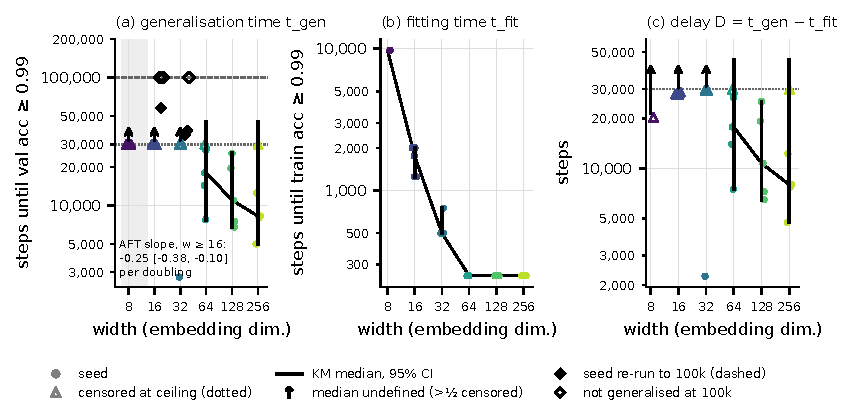
\includegraphics[width=\linewidth]{width_trends_main.pdf}
\caption{Timing versus width (one-layer transformer, addition mod 53, training fraction 0.4, AdamW, learning rate $10^{-3}$, weight decay 1; 5 seeds). (a) $\tgen$ over all runs; censored runs are open triangles at the ceiling and are kept. (b) $\tfit$ and (c) the delay exist only for runs that fit. Black: Kaplan--Meier median with 95\% bootstrap CI; arrow: median undefined. Shaded: widths below $w_{\min}$, excluded from the AFT slope printed below (a). Diamonds in (a): seeds 0--2 at $d=16,32$ re-run to a 100{,}000-step ceiling; the 30{,}000-step value there is a lower bound.}
\label{fig:width}
\end{figure}

\begin{table}[t]
\caption{Main sweep per width (5 seeds each). Regimes G/D/M/N: seeds that grok / generalise directly / memorise only / neither. Medians are Kaplan--Meier with 95\% bootstrap CIs over seeds; $>x$: median undefined (over half the seeds censored at 30,000 steps), $x$ = smallest observed value; $\infty$: CI bound undefined. Censored runs are never dropped.}
\label{tab:main}
\resizebox{\linewidth}{!}{%
\begin{tabular}{rrrrrrr}
\toprule
width & params & grokked & regimes G/D/M/N & KM median $t_{\mathrm{gen}}$ [95\% CI] & median $t_{\mathrm{fit}}$ [95\% CI] & KM median delay [95\% CI] \\
\midrule
8 & 1688 & 0/5 & 0/0/1/4 & $>$30,000 & 9,750 [9,750, 9,750] & $>$20,250 \\
16 & 4912 & 0/5 & 0/0/5/0 & $>$30,000 & 1,750 [1,250, 2,000] & $>$28,000 \\
32 & 15968 & 1/5 & 1/0/4/0 & $>$2,750 & 500 [500, 750] & $>$2,250 \\
64 & 56512 & 4/5 & 4/0/1/0 & 18,000 [7,750, $\infty$] & 250 [250, 250] & 17,750 [7,500, $\infty$] \\
128 & 211328 & 5/5 & 5/0/0/0 & 11,000 [6,750, 25,500] & 250 [250, 250] & 10,750 [6,500, 25,250] \\
256 & 815872 & 4/5 & 4/0/1/0 & 8,250 [5,000, $\infty$] & 250 [250, 250] & 8,000 [4,750, $\infty$] \\
\bottomrule
\end{tabular}}
\end{table}


\begin{figure}[t]
\centering
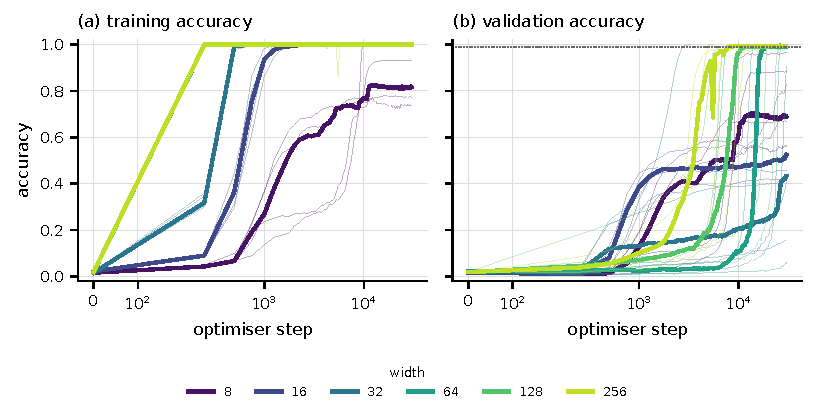
\includegraphics[width=\linewidth]{curves_main.pdf}
\caption{Training (a) and validation (b) accuracy during training for the main sweep (thin: single seeds, thick: median per width; logarithmic step axis).}
\label{fig:curves}
\end{figure}


\subsection{A2: the weight-norm mechanism is not supported; only the weight-decay scaling survives}
\label{sec:a2}
\textbf{(i) Weight decay.} Varying weight decay over $\{0.5,1,2\}$ at fixed learning rate, the slope of $\log D$ on $\log\mathrm{wd}$ is $-1.01$ $[-1.38,-0.66]$ at $d=128$ (consistent with $-1$) and $-0.61$ $[-1.05,-0.12]$ at $d=64$ (also consistent with $-1$, but wide and not close to it in its point estimate; Figure~\ref{fig:wd}a). At $d=64$ the dependence is not monotone: the median delay is 17{,}750 at wd=1 and 23{,}500 at wd=2, so the fitted slope rests on the wd=0.5 cell, which has a 60{,}000-step ceiling. Against the tolerance $|b+1|\le0.3$ neither interval lies wholly inside $[-1.3,-0.7]$, so we call the exponent of A2(i) \emph{inconclusive}; the direction (slope $<0$) is supported at both widths and not refuted.
\textbf{(ii) Mediation by norm.} We regress $\log D\sim\log\tfit+\log\lVert\theta_{\text{fit}}\rVert+\log d$ over all 66 transformer runs with $f=0.4$ (24 censored) and read ``width acts only through the norm'' as refuted if the width coefficient's interval excludes zero. The answer depends on the norm measure. With the \emph{total} $L_2$ norm the width coefficient is $-0.57$ $[-1.17,-0.13]$ (``refuted''), but the total norm grows with $\sqrt{\#\text{parameters}}$, hence about linearly in width, so it is collinear with width by construction (it rises from 23.5 at $d=8$ to 49.3 at $d=256$ while the delay shrinks). With the \emph{per-parameter RMS} norm ($L_2/\sqrt{\#\text{parameters}}$) the width coefficient is $+0.59$ $[-0.83,2.26]$: \emph{inconclusive}; the norm coefficient without width is $0.52$ $[0.13,0.89]$ (positive as predicted, but not beyond the negligibility band, inconclusive), against $-0.95$ $[-2.18,0.56]$ for the total norm. On the 26 main-sweep runs (five widths) the width coefficients have opposite signs under the two measures ($-1.70$ $[-4.26,-0.85]$ and $+3.68$ $[0.34,12.6]$), which shows that the regression cannot separate width from norm there. We therefore call A2(ii) \emph{inconclusive (refuted only under the total $L_2$ norm)}. The norm at $\tgen$ is contaminated by the outcome and is not used.
\textbf{(iii) Initialization scale.} Multiplying all initial parameters by $\alpha\in\{0.5,1,2\}$ raises the norm at fit (at $d=128$: 39.1, 42.8, 48.3), yet shortens generalization: the slope of $\log\tgen$ on $\log\alpha$ is $-0.57$ $[-0.95,-0.08]$ at $d=128$ and $-0.18$ $[-0.44,-0.01]$ at $d=32$ (borderline; Figure~\ref{fig:wd}b). This is a \emph{total} effect of initialization scale. At $d=128$ the norm at fit rises with $\alpha$ while $\tgen$ falls, a direction opposite to ``larger norm $\Rightarrow$ longer delay'' (direction-only: the interval is wholly below zero); under the strict band reading the verdict is \emph{inconclusive}, since the interval's upper end, $-0.08$, lies above the band edge $-0.10$. At $d=32$ the norm at fit is not monotone in $\alpha$ (34.0, 32.6, 34.8), so it is \emph{not tested} there. A norm-matched comparison was not achievable (the lowest norm at $d=128$, 39.1, still exceeds that of $d=32$ at $\alpha=1$, 32.6; $\alpha<0.5$ was not run), so mediation through the norm at fit remains untested by intervention.
Overall the account's norm-mediation mechanism is \emph{not supported}: no test supports it and two point against it, neither decisively (ii, iii); only the weight-decay scaling (i) survives, as a time scale not shown to run through the norm. The data do not separate an independent capacity effect (C1) from an initialization-scale-only effect (C2); and since the lr-rescaling check (3--5 seeds, mostly censored) cannot exclude that part of the width advantage depends on the fixed-learning-rate regime, C1 is at most one compatible reading.

\begin{figure}[t]
\centering
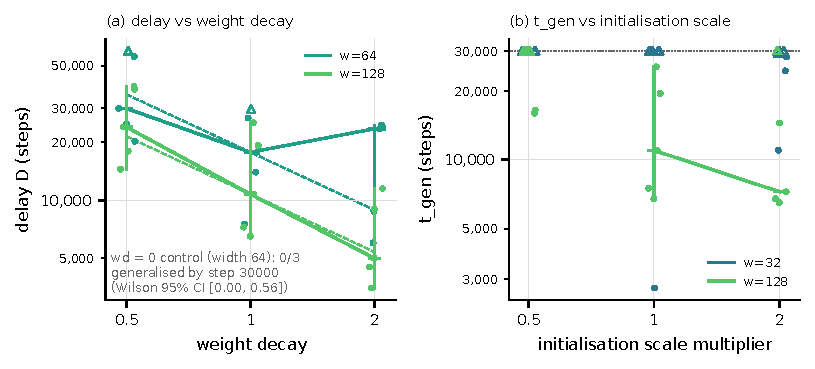
\includegraphics[width=\linewidth]{wd_alpha.pdf}
\caption{(a) Delay versus weight decay at widths 64 and 128 (dashed: AFT fit; slope $-1$ is the prediction); the wd=0 control (width 64) did not generalize in 0/3 runs. (b) $\tgen$ versus initialization-scale multiplier at widths 32 and 128. Markers as in Figure~\ref{fig:width}.}
\label{fig:wd}
\end{figure}

\subsection{A3 and scope: training fraction, parametrization, other tasks}
\label{sec:a3}
\textbf{Training fraction} (Figure~\ref{fig:frac}). At $f=0.25$ none of 5+5 runs at $d=32$ or $128$ generalize (mean final validation accuracy 0.02 and 0.10); at $f=0.4$, $1/5$ runs generalize at $d=32$ (Wilson $[0.04,0.62]$) versus $5/5$ at $d=128$ ($[0.57,1.0]$), the pre-stated pattern ``5/5 versus $\le1/5$'' holds, but with five seeds the Wilson intervals overlap, so this contrast alone is inconclusive; at $f=0.5$ all runs generalize at both widths, and the wider net is faster (KM median $\tgen$ 2{,}750 vs 9{,}000). The width contrast in the fraction that generalizes is thus seen at $f=0.4$ only, not at $0.25$ or $0.5$, so a critical-fraction shift with width is \emph{inconclusive}; by the Wilson rule, the supported contrasts are $f=0.5$ versus $0.25$ ($5/5$ versus $0/5$ at both widths) and $f=0.4$ versus $0.25$ at $d=128$, and at $f=0.5$ width still shortens $\tgen$. A finer fraction grid was not run. The delay does not vanish at $f=0.5$ (2{,}500 steps at $d=128$), so ``delay vanishes at large $f$'' is untested within our range.
\textbf{Weight decay zero} (width 64, 3 seeds): 0/3 generalize in 30{,}000 steps (Wilson upper bound $0.56$); this is consistent with A3 but has low power with three seeds, and is not a strong test.
\textbf{Parametrization} (learning rate multiplied by $\sqrt{64/d}$; 5 seeds at $d\in\{32,128\}$, 3 seeds at $d\in\{16,64,256\}$). At $d=32$ and $128$, $2/5$ and $3/5$ runs generalize (fixed rate: $1/5$ and $5/5$); the width contrast has Fisher $p=1.0$ in the scaled arm and $0.048$ at fixed rate. Over $d=16,\dots,256$ (3 seeds each) $0,0,3,1,1$ of 3 generalize against $0,0,3,3,2$ at fixed rate. The scaled-rate AFT slope is degenerate (10 of 15 runs censored, its bootstrap interval collapses to $[-0.05,0.00]$) and inconclusive, whereas the fixed-rate slope on the same 15 runs is $-0.20$ $[-0.32,-0.07]$. The width advantage at $d\ge128$ is thus weaker when the learning rate is scaled with width, but 30{,}000 steps censor most scaled-rate runs, so we can neither exclude nor confirm a dependence on the learning rate; all conclusions are stated \emph{under fixed learning rate, weight decay and initialization}.
\textbf{Other settings.} Two-hidden-layer MLPs show the same direction with faster generalization (KM median $\tgen$ 13{,}000, 8{,}000, 6{,}750, 6{,}000 at $d=32,64,128,256$; Table~\ref{tab:scope}, Figure~\ref{fig:scope}). Modular multiplication (2 widths $\times$ 3 seeds, $d=64,128$): all 6 runs generalize, KM median 22{,}500 versus 19{,}000 steps, CIs overlapping.

\begin{figure}[t]
\centering
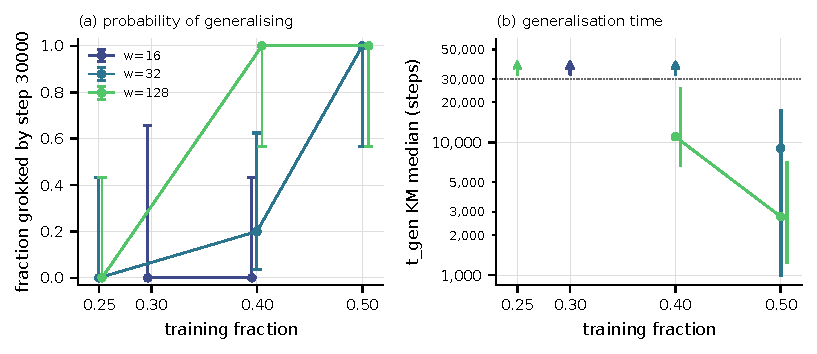
\includegraphics[width=\linewidth]{frac.pdf}
\caption{(a) Fraction of seeds generalizing within 30{,}000 steps versus training fraction, with Wilson 95\% intervals ($n=5$ per point, 2 at $f=0.3$, $d=16$). (b) KM median $\tgen$ versus fraction (arrow: undefined).}
\label{fig:frac}
\end{figure}

\subsection{Summary of verdicts}
\begin{table}[h!]
\centering\small
\caption{Pre-stated predictions and outcomes under the decision rule of Section~\ref{sec:method}. Evidence: \texttt{results/main\_stats.json}, \texttt{sens\_stats.json}, \texttt{mech\_stats.json}, \texttt{*\_cells.csv}.}
\label{tab:verdict}
\begin{tabular}{p{0.27\linewidth}p{0.18\linewidth}p{0.45\linewidth}}
\toprule
Prediction & Outcome & Basis \\
\midrule
A1 wider $\Rightarrow$ earlier $\tgen$ ($d\ge16$, fixed lr/wd/init) & supported & slope $-0.25$ $[-0.38,-0.10]$ (30k); $-0.41$ $[-0.57,-0.25]$ (100k, narrow widths); MLP $-0.38$; inconclusive on $d\ge32$ alone ($-0.31$ $[-0.62,0.12]$) \\
A2(i) $D\propto 1/\mathrm{wd}$ & direction supported; exponent inconclusive & $-1.01$ $[-1.38,-0.66]$ ($d=128$); $-0.61$ $[-1.05,-0.12]$ ($d=64$); neither inside $[-1.3,-0.7]$ \\
A2(ii) width acts only via $\tfit$ and norm at fit & inconclusive (refuted only under total $L_2$) & width coefficient $-0.57$ $[-1.17,-0.13]$ (total $L_2$); $+0.59$ $[-0.83,2.26]$ (per-parameter RMS); the two norms are collinear with width differently \\
A2(iii) init scale / norm matching & direction-only against ($d=128$); verdict inconclusive; not tested at $d=32$ & $\log\tgen$ slope in $\log\alpha$ $-0.57$ $[-0.95,-0.08]$ ($d=128$), norm rises with $\alpha$; norm matching not achievable \\
A2 mechanism overall & not supported & no test supports it; two point against, neither decisive \\
A3 critical fraction shifts with width & inconclusive & 1/5 vs 5/5 at $f=0.4$; 0/5 vs 0/5 at $0.25$, 5/5 vs 5/5 at $0.5$ \\
A3 no grokking at wd=0 & consistent, low power & 0/3 (Wilson upper bound 0.56) \\
A3 delay vanishes at large $f$ & untested & max $f=0.5$ \\
Parametrization (lr $\propto 1/\sqrt d$) & open (flag) & $d=128$ vs $32$: 3/5 vs 2/5 (scaled), 5/5 vs 1/5 (fixed), Fisher $p=1.0$ vs $0.048$; scaled AFT slope inconclusive (10/15 censored) \\
C3 no width effect & refuted (fixed regime) & A1 slope, JT test \\
C1 vs C2 & not separable; C1 one compatible reading & A2(ii), A2(iii), lr-rescaling \\
\bottomrule
\end{tabular}
\end{table}

\section{Discussion and limitations}
\label{sec:disc}
Under fixed learning rate, weight decay and initialization, a wider transformer generalizes sooner on this task, and the delay's inverse dependence on weight decay is consistent with a weight-decay-driven cleanup time scale. The weight-norm mechanism we proposed for the width effect is not supported: whether width keeps a coefficient after conditioning on the norm at fit depends on the norm measure (yes for the total $L_2$ norm, which is collinear with width; inconclusive for the per-parameter RMS norm), and at $d=128$ the intervention that raises the norm at fit (larger initial scale) shortens the delay; a norm-matched test was not feasible. The initial-scale result is a total effect, compatible with larger initial scale favoring richer feature learning \citep{kumar2024grokking,liu2023omnigrok}, but we did not test this, and we cannot separate an independent capacity effect from an initialization-scale effect.

\paragraph{Limitations and failure cases.}
(1) One task family and prime ($p=53$), mostly addition; multiplication with 3 seeds and 2 widths.
(2) Width range $8$--$256$ at one layer; depth and the number of heads were not varied (heads change from 1 to 4 between $d=8$ and $d\ge16$).
(3) Five seeds per cell (3 for several controls); intervals are wide, and several verdicts are ``inconclusive'' or ``narrow''. The $d=16$ and $d=32$ medians are undefined at the 30{,}000-step ceiling.
(4) Hyperparameters are fixed across width; the learning-rate-scaled check weakens the width advantage at $d\ge128$ but is mostly censored at 30{,}000 steps (3--5 seeds), so it neither excludes nor confirms a dependence, and we did not tune each width.
(5) A1 uses a lognormal AFT model; its CIs are bootstrap intervals conditional on that model. The logging interval of 250 steps bounds the resolution of $\tfit$ (which is at the resolution for $d\ge64$).
(6) Not run: the split-seed versus init-seed separation, a second prime, the Nanda-configuration anchor ($p=113$), $\alpha<0.5$, a finer training-fraction grid, depth, optimizer and batch-size variation, and a norm-matched comparison; the exact $1.0$-threshold check covers only $d\ge64$ (inconclusive), and $0.9$/$0.95$ thresholds are exact. The 30{,}000-step cells at narrow widths are lower bounds on $\tgen$.
(7) The plan was amended after partial data were seen (Section~\ref{sec:method}); the A2 regression is collinear in width and norm, the negligibility bands were fixed after the results were seen, and the post-hoc outcome classification is exploratory.
(8) We did not use mechanistic diagnostics (Fourier or restricted-loss analyses), so claims about circuits are interpretations, not findings.

\textbf{Reproducibility.} Code, run logs and the artifact map are in the delivered repository (\texttt{paper/REPRODUCE.md}); data are generated in memory.

\bibliographystyle{plainnat}
\bibliography{references}

\appendix
\section{Additional figures and tables}
\label{app:figs}
\begin{figure}[h]
\centering
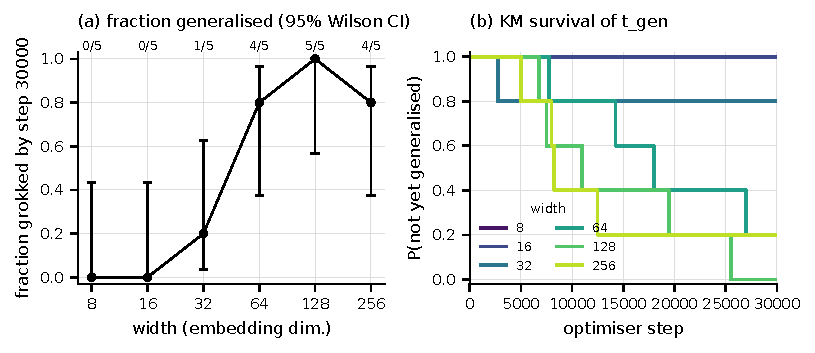
\includegraphics[width=\linewidth]{grok_survival_main.pdf}
\caption{Probability of generalizing and survival of $\tgen$ by width.}
\end{figure}
\begin{figure}[h]
\centering
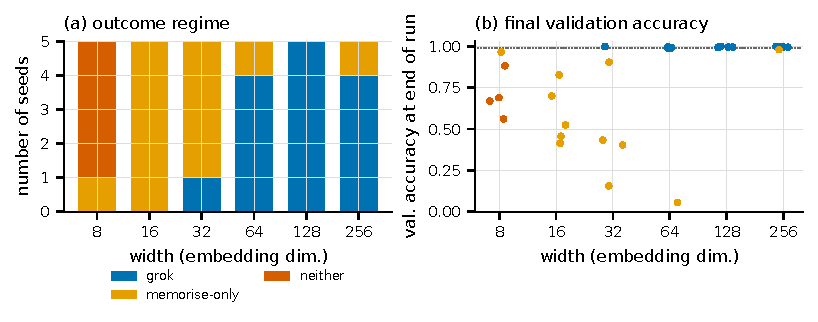
\includegraphics[width=\linewidth]{regimes_main.pdf}
\caption{Outcome regimes per width.}
\end{figure}
\begin{figure}[h]
\centering
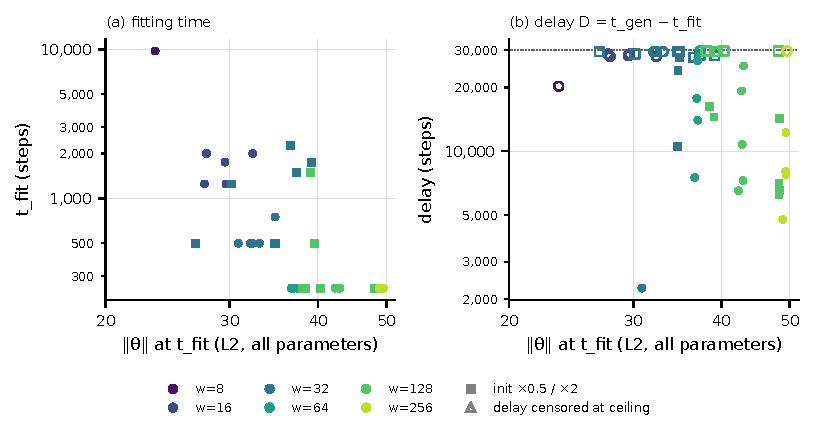
\includegraphics[width=\linewidth]{mechanism.pdf}
\caption{Weight norm at the time the training set is fitted versus (a) $\tfit$ and (b) the delay, one point per run (colour: width). Circles: default initialization; squares: initialization scaled by 0.5 or 2. Open markers in (b): runs not generalized within the ceiling. Only runs that fitted the training set appear. Norm is the total $L_2$ norm.}
\end{figure}
\begin{figure}[h]
\centering
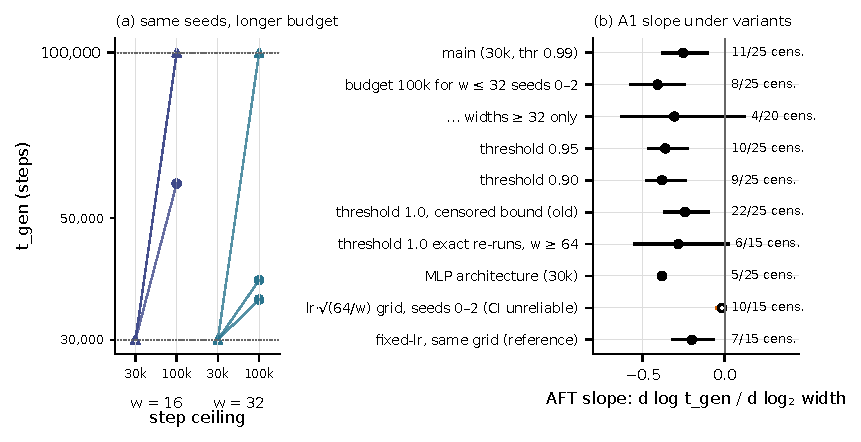
\includegraphics[width=\linewidth]{budget.pdf}
\caption{Sensitivity of the width effect to step budget, threshold and architecture. (a) Seeds 0--2 at widths 16 and 32 under the 30{,}000-step ceiling (main) and a 100{,}000-step ceiling (long; identical through step 30{,}000); open triangles: not generalized at that ceiling. (b) Censoring-aware lognormal AFT slope of $\log\tgen$ on $\log_2 d$ over $d\ge w_{\min}$ with 95\% bootstrap CIs over runs (negative: wider generalizes sooner); right: censored/total runs. The first threshold-1.0 row is a censored bound only; the exact row re-ran widths $\ge64$ to validation accuracy 1.0. The learning-rate-scaled row is the AFT slope over widths 16--256 (seeds 0--2) with 10 of 15 runs censored, so its interval collapses toward 0 and is not evidence of no effect; the row beneath is the fixed-rate slope on the same runs.}
\label{fig:budget}
\end{figure}
\begin{figure}[h]
\centering
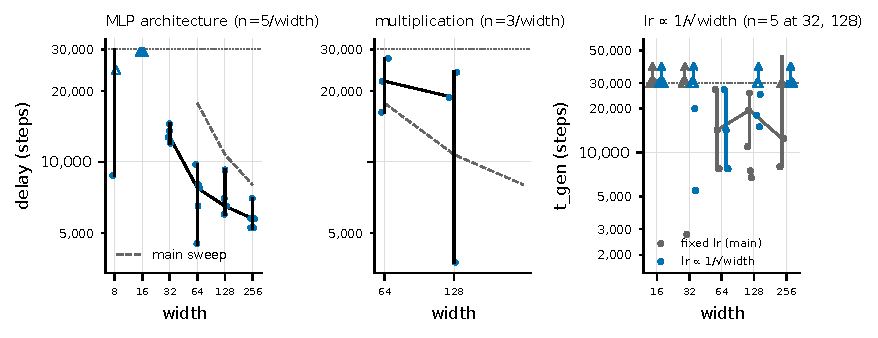
\includegraphics[width=\linewidth]{scope.pdf}
\caption{Secondary conditions. (a, b) Delay versus width for the MLP and for multiplication, shared $y$-axis. Filled: generalized; open triangle: right-censored at the ceiling. Black: Kaplan--Meier median with 95\% bootstrap CI; dashed grey: main-sweep medians. (c) Learning rate scaled as $\mathrm{lr}\sqrt{64/d}$ (blue) against fixed-rate main-sweep runs on the same seeds (grey), $\tgen$ on the $y$-axis because most scaled-rate runs do not generalize. Points: seeds 0--4 at $d=32,128$ and seeds 0--2 at $d=16,64,256$; lines: KM median over seeds 0--2.}
\label{fig:scope}
\end{figure}
\begin{table}[t]
\caption{Scope sweeps: same columns as Table~\ref{tab:main} for secondary conditions.}
\label{tab:scope}
\resizebox{\linewidth}{!}{%
\begin{tabular}{rrrrrrrr}
\toprule
sweep & condition & width & grokked & regimes G/D/M/N & KM median $t_{\mathrm{gen}}$ [95\% CI] & median $t_{\mathrm{fit}}$ [95\% CI] & KM median delay [95\% CI] \\
\midrule
frac & train frac 0.25 & 32 & 0/5 & 0/0/5/0 & $>$30,000 & 500 [500, 500] & $>$29,500 \\
frac & train frac 0.25 & 128 & 0/5 & 0/0/5/0 & $>$30,000 & 250 [250, 250] & $>$29,750 \\
frac & train frac 0.3 & 16 & 0/2 & 0/0/2/0 & $>$30,000 & 3,125 [1,250, 5,000] & $>$25,000 \\
frac & train frac 0.5 & 32 & 5/5 & 5/0/0/0 & 9,000 [1,000, 17,250] & 750 [500, 1,250] & 8,250 [500, 16,000] \\
frac & train frac 0.5 & 128 & 5/5 & 5/0/0/0 & 2,750 [1,250, 7,000] & 250 [250, 250] & 2,500 [1,000, 6,750] \\
wd & wd 0.5 & 64 & 4/5 & 4/0/1/0 & 30,250 [20,500, $\infty$] & 250 [250, 250] & 30,000 [20,250, $\infty$] \\
wd & wd 0.5 & 128 & 5/5 & 5/0/0/0 & 24,250 [14,750, 39,250] & 250 [250, 250] & 24,000 [14,500, 39,000] \\
wd & wd 2 & 64 & 5/5 & 5/0/0/0 & 24,000 [6,250, 25,000] & 500 [250, 500] & 23,500 [6,000, 24,500] \\
wd & wd 2 & 128 & 5/5 & 5/0/0/0 & 5,250 [3,750, 11,750] & 250 [250, 250] & 5,000 [3,500, 11,500] \\
wd0 & wd 0 & 64 & 0/3 & 0/0/3/0 & $>$30,000 & 250 [250, 250] & $>$29,750 \\
alpha & init $\times$0.5 & 32 & 0/5 & 0/0/5/0 & $>$30,000 & 1,500 [500, 2,250] & $>$27,750 \\
alpha & init $\times$2 & 32 & 3/5 & 3/0/2/0 & 28,250 [11,000, $\infty$] & 500 [500, 500] & 27,750 [10,500, $\infty$] \\
alpha & init $\times$0.5 & 128 & 2/5 & 2/0/3/0 & $>$16,000 & 250 [250, 1,500] & $>$14,500 \\
alpha & init $\times$2 & 128 & 4/5 & 4/0/1/0 & 7,250 [6,500, $\infty$] & 250 [250, 250] & 7,000 [6,250, $\infty$] \\
lrscale & lr $\propto 1/\sqrt{w}$ (ref 64) & 32 & 2/5 & 2/0/3/0 & $>$5,500 & 500 [500, 500] & $>$5,000 \\
lrscale & lr $\propto 1/\sqrt{w}$ (ref 64) & 128 & 3/5 & 3/0/2/0 & 25,000 [15,000, $\infty$] & 250 [250, 250] & 24,750 [14,750, $\infty$] \\
lrscale2 & lr $\propto 1/\sqrt{w}$ (ref 64) & 16 & 0/3 & 0/0/3/0 & $>$30,000 & 1,000 [1,000, 1,000] & $>$29,000 \\
lrscale2 & lr $\propto 1/\sqrt{w}$ (ref 64) & 64 & 3/3 & 3/0/0/0 & 14,250 [7,750, 27,000] & 250 [250, 250] & 14,000 [7,500, 26,750] \\
lrscale2 & lr $\propto 1/\sqrt{w}$ (ref 64) & 256 & 1/3 & 1/0/2/0 & $>$29,750 & 250 [250, 250] & $>$29,500 \\
mlp & arch mlp & 8 & 1/5 & 1/0/1/3 & $>$10,750 & 3,750 [2,000, 5,500] & 8,750 [8,750, $\infty$] \\
mlp & arch mlp & 16 & 0/5 & 0/0/5/0 & $>$30,000 & 750 [750, 750] & $>$29,250 \\
mlp & arch mlp & 32 & 5/5 & 5/0/0/0 & 13,000 [12,250, 14,750] & 250 [250, 250] & 12,750 [12,000, 14,500] \\
mlp & arch mlp & 64 & 5/5 & 5/0/0/0 & 8,000 [4,750, 10,000] & 250 [250, 250] & 7,750 [4,500, 9,750] \\
mlp & arch mlp & 128 & 5/5 & 5/0/0/0 & 6,750 [6,250, 9,500] & 250 [250, 250] & 6,500 [6,000, 9,250] \\
mlp & arch mlp & 256 & 5/5 & 5/0/0/0 & 6,000 [5,500, 7,250] & 250 [250, 250] & 5,750 [5,250, 7,000] \\
mul & op mul & 64 & 3/3 & 3/0/0/0 & 22,500 [16,750, 28,000] & 500 [500, 500] & 22,000 [16,250, 27,500] \\
mul & op mul & 128 & 3/3 & 3/0/0/0 & 19,000 [4,000, 24,250] & 250 [250, 250] & 18,750 [3,750, 24,000] \\
\bottomrule
\end{tabular}}
\end{table}

\begin{table}[t]
\caption{Trend of generalisation time with width. JT: Jonckheere--Terpstra-type statistic, negative = faster for wider nets, two-sided permutation $p$, censoring-aware. AFT: lognormal accelerated-failure-time slope of $\log t_{gen}$ on $\log_2$ width, 95\% bootstrap CI over seeds (the plan's A1 estimand; negative = wider nets generalise sooner). Verdict: the plan's rule with the negligible bands of story-repo's \texttt{VERDICTS.md}, as written by the analysis position into the stats files (bands set after the results were seen). The scaled-learning-rate row is censored for 10 of 15 runs; with most runs sharing one censoring time the bootstrap CI collapses toward 0, so an interval inside the negligible band is not evidence of no effect (the verdict is inconclusive, not null).}
\label{tab:trend}
\resizebox{\linewidth}{!}{%
\begin{tabular}{llllll}
\toprule
sweep & condition & endpoint & estimate & test & verdict \\
\midrule
main & transformer, add mod 53, $f$=0.4 & t\_gen, all runs & JT = -199 & permutation p = 0.0002 & -- \\
main & transformer, add mod 53, $f$=0.4 & log t\_gen per doubling (AFT, w $\geq$ 16) & -0.25 [-0.38, -0.10] & n = 25 (11 censored) & supported \\
main & transformer, add mod 53, $f$=0.4 & delay, runs that fit & JT = -141 & permutation p = 0.0006 & -- \\
mlp & MLP, add mod 53, $f$=0.4 & t\_gen, all runs & JT = -296 & permutation p = 0.0002 & -- \\
mlp & MLP, add mod 53, $f$=0.4 & log t\_gen per doubling (AFT, w $\geq$ 16) & -0.38 [-0.40, -0.36] & n = 25 (5 censored) & supported \\
mlp & MLP, add mod 53, $f$=0.4 & delay, runs that fit & JT = -232 & permutation p = 0.0002 & -- \\
sensitivity & 100k-step ceiling for w $\leq$ 32, seeds 0--2 & log t\_gen per doubling (AFT, w $\geq$ 16) & -0.41 [-0.57, -0.25] & n = 25 (8 censored) & supported \\
sensitivity & same, widths $\geq$ 32 only & log t\_gen per doubling (AFT, w $\geq$ 32) & -0.31 [-0.62, 0.12] & n = 20 (4 censored) & inconclusive \\
sensitivity & threshold 1.0 (bound only) & log t\_gen per doubling (AFT, w $\geq$ 16) & -0.24 [-0.37, -0.10] & n = 25 (22 censored) & inconclusive \\
sensitivity & threshold 0.90 & log t\_gen per doubling (AFT, w $\geq$ 16) & -0.38 [-0.48, -0.24] & n = 25 (9 censored) & supported \\
sensitivity & threshold 0.95 & log t\_gen per doubling (AFT, w $\geq$ 16) & -0.36 [-0.46, -0.23] & n = 25 (10 censored) & supported \\
sensitivity & threshold 1.0, exact re-runs (thr1) & log t\_gen per doubling (AFT, w $\geq$ 64) & -0.28 [-0.55, 0.02] & n = 15 (6 censored) & inconclusive \\
sensitivity & lr $\propto 1/\sqrt{w}$, seeds 0--2, w 16--256 & log t\_gen per doubling (AFT, w $\geq$ 16); CI unreliable & -0.02 [-0.05, -0.00] & n = 15 (10 censored) & inconclusive \\
sensitivity & fixed lr, same seeds and widths (reference) & log t\_gen per doubling (AFT, w $\geq$ 16) & -0.20 [-0.32, -0.07] & n = 15 (7 censored) & -- \\
\bottomrule
\end{tabular}}
\end{table}

\begin{table}[t]
\caption{A2(ii): regression of $\log D$ (lognormal AFT, censored runs kept) on $\log t_{fit}$ and the weight norm at $t_{fit}$ ($\pm$ $\log$ width), with the norm measured as the total L2 norm of all parameters and as the per-parameter RMS (total/$\sqrt{\mathrm{params}}$; total L2 grows with width by construction). Cells: coefficient [95\% bootstrap CI] and the verdict under the plan's bands (norm coefficient predicted $>0$: supported if the CI lies above 0.25, refuted if below 0.25). For the width row the verdict is for ``width acts only through $t_{fit}$ and the norm'' (refuted if the width CI excludes 0). Width and norm are collinear, so these are supporting only. Regressions on the norm at $t_{gen}$ are outcome-contaminated and not shown.}
\label{tab:mech}
\resizebox{\linewidth}{!}{%
\begin{tabular}{llllll}
\toprule
sample & coefficient & total L2 [CI] & total L2 verdict & RMS [CI] & RMS verdict \\
\midrule
main sweep (n=26, 12 cens.) & $\log$ norm (given $\log t_{fit}$) & -0.96 [-3.59, 1.55] & inconclusive & 0.51 [-0.13, 1.02] & inconclusive \\
main sweep (n=26, 12 cens.) & $\log$ norm (given $\log t_{fit}$, $\log$ width) & 6.73 [1.40, 19.84] & supported & 5.26 [1.26, 16.84] & supported \\
main sweep (n=26, 12 cens.) & $\log$ width (given $\log t_{fit}$, $\log$ norm) & -1.70 [-4.26, -0.85] & refuted & 3.68 [0.34, 12.65] & refuted \\
all $f$=0.4 runs (n=66, 24 cens.) & $\log$ norm (given $\log t_{fit}$) & -0.95 [-2.18, 0.56] & inconclusive & 0.52 [0.13, 0.89] & inconclusive \\
all $f$=0.4 runs (n=66, 24 cens.) & $\log$ norm (given $\log t_{fit}$, $\log$ width) & 1.04 [-0.94, 3.74] & inconclusive & 1.28 [-0.50, 3.47] & inconclusive \\
all $f$=0.4 runs (n=66, 24 cens.) & $\log$ width (given $\log t_{fit}$, $\log$ norm) & -0.57 [-1.17, -0.13] & refuted & 0.59 [-0.83, 2.26] & inconclusive \\
\bottomrule
\end{tabular}}
\end{table}

\begin{table}[t]
\caption{A2(i) weight-decay exponent and A2(iii) init-scale effect (lognormal AFT, censored runs kept; the $wd=0.5$ runs have a 60,000-step ceiling). A2(i): supported if the CI lies inside $[-1.3,-0.7]$, refuted if wholly outside. A2(iii): the mediation account predicts a positive slope where the norm at fit rises with $\alpha$ (supported if lo $>0.10$, refuted if hi $<-0.10$; ``not tested'' where the norm at fit is not monotone in $\alpha$); the direction-only column asks only whether hi $<0$.}
\label{tab:wdalpha}
\resizebox{\linewidth}{!}{%
\begin{tabular}{llllll}
\toprule
estimand & setting & n (censored) & estimate [CI] & verdict & direction-only \\
\midrule
A2(i): $d\log D/d\log wd$ (predicted $-1$) & width 64, wd $\in$ {0.5, 1, 2} & 15 (2) & -0.61 [-1.05, -0.12] & inconclusive & -- \\
A2(i): $d\log D/d\log wd$ (predicted $-1$) & width 128, wd $\in$ {0.5, 1, 2} & 15 (0) & -1.01 [-1.38, -0.66] & inconclusive & -- \\
A2(iii): $d\log t_{gen}/d\log\alpha$ (init scale) & width 32, $\alpha\in${0.5, 1, 2} & 15 (11) & -0.18 [-0.44, -0.01] & not tested & not tested \\
A2(iii): $d\log t_{gen}/d\log\alpha$ (init scale) & width 128, $\alpha\in${0.5, 1, 2} & 15 (4) & -0.57 [-0.95, -0.08] & inconclusive & refuted \\
\bottomrule
\end{tabular}}
\end{table}


\section{Use of LLM agents}
\label{app:llm}
The study (plan, code, runs, analysis and manuscript) was carried out by LLM-based agents working as separate roles (planning, experiments, figures, venue, writing, review) under a human-specified task. They are not part of the studied method. All numbers in this paper come from the shipped run logs and analysis scripts; the agents' roles and hand-offs are recorded in the delivery repository's issue and pull-request history.

\newpage
\section*{NeurIPS Paper Checklist}




\begin{enumerate}

\item {\bf Claims}
    \item[] Question: Do the main claims made in the abstract and introduction accurately reflect the paper's contributions and scope?
    \item[] Answer: \answerYes{} % Replace by \answerYes{}, \answerNo{}, or \answerNA{}.
    \item[] Justification: Abstract and Section~1 state the task, width range, single prime, and that outcomes are supported, refuted or inconclusive; Table~\ref{tab:verdict} lists each.
    \item[] Guidelines:
    \begin{itemize}
        \item The answer \answerNA{} means that the abstract and introduction do not include the claims made in the paper.
        \item The abstract and/or introduction should clearly state the claims made, including the contributions made in the paper and important assumptions and limitations. A \answerNo{} or \answerNA{} answer to this question will not be perceived well by the reviewers. 
        \item The claims made should match theoretical and experimental results, and reflect how much the results can be expected to generalize to other settings. 
        \item It is fine to include aspirational goals as motivation as long as it is clear that these goals are not attained by the paper. 
    \end{itemize}

\item {\bf Limitations}
    \item[] Question: Does the paper discuss the limitations of the work performed by the authors?
    \item[] Answer: \answerYes{} % Replace by \answerYes{}, \answerNo{}, or \answerNA{}.
    \item[] Justification: Section~\ref{sec:disc} lists limitations (one task family and prime, narrow width range, few seeds, fixed hyperparameters, censoring, post-hoc plan amendments, no mechanistic analysis).
    \item[] Guidelines:
    \begin{itemize}
        \item The answer \answerNA{} means that the paper has no limitation while the answer \answerNo{} means that the paper has limitations, but those are not discussed in the paper. 
        \item The authors are encouraged to create a separate ``Limitations'' section in their paper.
        \item The paper should point out any strong assumptions and how robust the results are to violations of these assumptions (e.g., independence assumptions, noiseless settings, model well-specification, asymptotic approximations only holding locally). The authors should reflect on how these assumptions might be violated in practice and what the implications would be.
        \item The authors should reflect on the scope of the claims made, e.g., if the approach was only tested on a few datasets or with a few runs. In general, empirical results often depend on implicit assumptions, which should be articulated.
        \item The authors should reflect on the factors that influence the performance of the approach. For example, a facial recognition algorithm may perform poorly when image resolution is low or images are taken in low lighting. Or a speech-to-text system might not be used reliably to provide closed captions for online lectures because it fails to handle technical jargon.
        \item The authors should discuss the computational efficiency of the proposed algorithms and how they scale with dataset size.
        \item If applicable, the authors should discuss possible limitations of their approach to address problems of privacy and fairness.
        \item While the authors might fear that complete honesty about limitations might be used by reviewers as grounds for rejection, a worse outcome might be that reviewers discover limitations that aren't acknowledged in the paper. The authors should use their best judgment and recognize that individual actions in favor of transparency play an important role in developing norms that preserve the integrity of the community. Reviewers will be specifically instructed to not penalize honesty concerning limitations.
    \end{itemize}

\item {\bf Theory assumptions and proofs}
    \item[] Question: For each theoretical result, does the paper provide the full set of assumptions and a complete (and correct) proof?
    \item[] Answer: \answerNA{} % Replace by \answerYes{}, \answerNo{}, or \answerNA{}.
    \item[] Justification: The paper has no theorems; the time-scale account in Section~\ref{sec:method} is a heuristic stated as testable predictions, not a proof.
    \item[] Guidelines:
    \begin{itemize}
        \item The answer \answerNA{} means that the paper does not include theoretical results. 
        \item All the theorems, formulas, and proofs in the paper should be numbered and cross-referenced.
        \item All assumptions should be clearly stated or referenced in the statement of any theorems.
        \item The proofs can either appear in the main paper or the supplemental material, but if they appear in the supplemental material, the authors are encouraged to provide a short proof sketch to provide intuition. 
        \item Inversely, any informal proof provided in the core of the paper should be complemented by formal proofs provided in appendix or supplemental material.
        \item Theorems and Lemmas that the proof relies upon should be properly referenced. 
    \end{itemize}

    \item {\bf Experimental result reproducibility}
    \item[] Question: Does the paper fully disclose all the information needed to reproduce the main experimental results of the paper to the extent that it affects the main claims and/or conclusions of the paper (regardless of whether the code and data are provided or not)?
    \item[] Answer: \answerYes{} % Replace by \answerYes{}, \answerNo{}, or \answerNA{}.
    \item[] Justification: Sections~\ref{sec:method}--\ref{sec:exp} and \texttt{paper/REPRODUCE.md} give architecture, optimizer, learning rate, weight decay, full-batch training, $p$, training fraction, seeds, step budgets and the $t_{\text{fit}}/t_{\text{gen}}$ definition with its censoring rule.
    \item[] Guidelines:
    \begin{itemize}
        \item The answer \answerNA{} means that the paper does not include experiments.
        \item If the paper includes experiments, a \answerNo{} answer to this question will not be perceived well by the reviewers: Making the paper reproducible is important, regardless of whether the code and data are provided or not.
        \item If the contribution is a dataset and\slash or model, the authors should describe the steps taken to make their results reproducible or verifiable. 
        \item Depending on the contribution, reproducibility can be accomplished in various ways. For example, if the contribution is a novel architecture, describing the architecture fully might suffice, or if the contribution is a specific model and empirical evaluation, it may be necessary to either make it possible for others to replicate the model with the same dataset, or provide access to the model. In general. releasing code and data is often one good way to accomplish this, but reproducibility can also be provided via detailed instructions for how to replicate the results, access to a hosted model (e.g., in the case of a large language model), releasing of a model checkpoint, or other means that are appropriate to the research performed.
        \item While NeurIPS does not require releasing code, the conference does require all submissions to provide some reasonable avenue for reproducibility, which may depend on the nature of the contribution. For example
        \begin{enumerate}
            \item If the contribution is primarily a new algorithm, the paper should make it clear how to reproduce that algorithm.
            \item If the contribution is primarily a new model architecture, the paper should describe the architecture clearly and fully.
            \item If the contribution is a new model (e.g., a large language model), then there should either be a way to access this model for reproducing the results or a way to reproduce the model (e.g., with an open-source dataset or instructions for how to construct the dataset).
            \item We recognize that reproducibility may be tricky in some cases, in which case authors are welcome to describe the particular way they provide for reproducibility. In the case of closed-source models, it may be that access to the model is limited in some way (e.g., to registered users), but it should be possible for other researchers to have some path to reproducing or verifying the results.
        \end{enumerate}
    \end{itemize}


\item {\bf Open access to data and code}
    \item[] Question: Does the paper provide open access to the data and code, with sufficient instructions to faithfully reproduce the main experimental results, as described in supplemental material?
    \item[] Answer: \answerYes{} % Replace by \answerYes{}, \answerNo{}, or \answerNA{}.
    \item[] Justification: Data are generated in memory (no download); all code, run logs and aggregated results are in the delivered repository with run commands in \texttt{paper/REPRODUCE.md}. No identifying URLs are given in the anonymized PDF.
    \item[] Guidelines:
    \begin{itemize}
        \item The answer \answerNA{} means that paper does not include experiments requiring code.
        \item Please see the NeurIPS code and data submission guidelines (\url{https://neurips.cc/public/guides/CodeSubmissionPolicy}) for more details.
        \item While we encourage the release of code and data, we understand that this might not be possible, so \answerNo{} is an acceptable answer. Papers cannot be rejected simply for not including code, unless this is central to the contribution (e.g., for a new open-source benchmark).
        \item The instructions should contain the exact command and environment needed to run to reproduce the results. See the NeurIPS code and data submission guidelines (\url{https://neurips.cc/public/guides/CodeSubmissionPolicy}) for more details.
        \item The authors should provide instructions on data access and preparation, including how to access the raw data, preprocessed data, intermediate data, and generated data, etc.
        \item The authors should provide scripts to reproduce all experimental results for the new proposed method and baselines. If only a subset of experiments are reproducible, they should state which ones are omitted from the script and why.
        \item At submission time, to preserve anonymity, the authors should release anonymized versions (if applicable).
        \item Providing as much information as possible in supplemental material (appended to the paper) is recommended, but including URLs to data and code is permitted.
    \end{itemize}


\item {\bf Experimental setting/details}
    \item[] Question: Does the paper specify all the training and test details (e.g., data splits, hyperparameters, how they were chosen, type of optimizer) necessary to understand the results?
    \item[] Answer: \answerYes{} % Replace by \answerYes{}, \answerNo{}, or \answerNA{}.
    \item[] Justification: Section~\ref{sec:method} (split rule: random train/validation split of all $p^2$ pairs per seed; no hyperparameter search, hyperparameters fixed a priori and varied only as stated) and \texttt{REPRODUCE.md}.
    \item[] Guidelines:
    \begin{itemize}
        \item The answer \answerNA{} means that the paper does not include experiments.
        \item The experimental setting should be presented in the core of the paper to a level of detail that is necessary to appreciate the results and make sense of them.
        \item The full details can be provided either with the code, in appendix, or as supplemental material.
    \end{itemize}

\item {\bf Experiment statistical significance}
    \item[] Question: Does the paper report error bars suitably and correctly defined or other appropriate information about the statistical significance of the experiments?
    \item[] Answer: \answerYes{} % Replace by \answerYes{}, \answerNo{}, or \answerNA{}.
    \item[] Justification: Every timing estimate carries a bootstrap CI (KM medians), slopes carry bootstrap CIs from a censoring-aware AFT model, fractions carry Wilson intervals; the method and its assumptions (lognormal AFT, 2000/500 resamples) are in Section~\ref{sec:method}, and censored runs are kept.
    \item[] Guidelines:
    \begin{itemize}
        \item The answer \answerNA{} means that the paper does not include experiments.
        \item The authors should answer \answerYes{} if the results are accompanied by error bars, confidence intervals, or statistical significance tests, at least for the experiments that support the main claims of the paper.
        \item The factors of variability that the error bars are capturing should be clearly stated (for example, train/test split, initialization, random drawing of some parameter, or overall run with given experimental conditions).
        \item The method for calculating the error bars should be explained (closed form formula, call to a library function, bootstrap, etc.)
        \item The assumptions made should be given (e.g., Normally distributed errors).
        \item It should be clear whether the error bar is the standard deviation or the standard error of the mean.
        \item It is OK to report 1-sigma error bars, but one should state it. The authors should preferably report a 2-sigma error bar than state that they have a 96\% CI, if the hypothesis of Normality of errors is not verified.
        \item For asymmetric distributions, the authors should be careful not to show in tables or figures symmetric error bars that would yield results that are out of range (e.g., negative error rates).
        \item If error bars are reported in tables or plots, the authors should explain in the text how they were calculated and reference the corresponding figures or tables in the text.
    \end{itemize}

\item {\bf Experiments compute resources}
    \item[] Question: For each experiment, does the paper provide sufficient information on the computer resources (type of compute workers, memory, time of execution) needed to reproduce the experiments?
    \item[] Answer: \answerYes{} % Replace by \answerYes{}, \answerNo{}, or \answerNA{}.
    \item[] Justification: Run times, hardware and core usage are in \texttt{REPRODUCE.md}: one CPU core per run, 5--120 minutes per run depending on width and load, about 44 hours of run time in total; peak memory was not logged.
    \item[] Guidelines:
    \begin{itemize}
        \item The answer \answerNA{} means that the paper does not include experiments.
        \item The paper should indicate the type of compute workers CPU or GPU, internal cluster, or cloud provider, including relevant memory and storage.
        \item The paper should provide the amount of compute required for each of the individual experimental runs as well as estimate the total compute. 
        \item The paper should disclose whether the full research project required more compute than the experiments reported in the paper (e.g., preliminary or failed experiments that didn't make it into the paper). 
    \end{itemize}
    
\item {\bf Code of ethics}
    \item[] Question: Does the research conducted in the paper conform, in every respect, with the NeurIPS Code of Ethics \url{https://neurips.cc/public/EthicsGuidelines}?
    \item[] Answer: \answerYes{} % Replace by \answerYes{}, \answerNo{}, or \answerNA{}.
    \item[] Justification: The work uses only synthetic modular-arithmetic data, no human subjects, and follows the NeurIPS Code of Ethics.
    \item[] Guidelines:
    \begin{itemize}
        \item The answer \answerNA{} means that the authors have not reviewed the NeurIPS Code of Ethics.
        \item If the authors answer \answerNo, they should explain the special circumstances that require a deviation from the Code of Ethics.
        \item The authors should make sure to preserve anonymity (e.g., if there is a special consideration due to laws or regulations in their jurisdiction).
    \end{itemize}


\item {\bf Broader impacts}
    \item[] Question: Does the paper discuss both potential positive societal impacts and negative societal impacts of the work performed?
    \item[] Answer: \answerNA{} % Replace by \answerYes{}, \answerNo{}, or \answerNA{}.
    \item[] Justification: The study is foundational, on a synthetic task, with no direct societal application; we see no specific positive or negative societal impact.
    \item[] Guidelines:
    \begin{itemize}
        \item The answer \answerNA{} means that there is no societal impact of the work performed.
        \item If the authors answer \answerNA{} or \answerNo, they should explain why their work has no societal impact or why the paper does not address societal impact.
        \item Examples of negative societal impacts include potential malicious or unintended uses (e.g., disinformation, generating fake profiles, surveillance), fairness considerations (e.g., deployment of technologies that could make decisions that unfairly impact specific groups), privacy considerations, and security considerations.
        \item The conference expects that many papers will be foundational research and not tied to particular applications, let alone deployments. However, if there is a direct path to any negative applications, the authors should point it out. For example, it is legitimate to point out that an improvement in the quality of generative models could be used to generate Deepfakes for disinformation. On the other hand, it is not needed to point out that a generic algorithm for optimizing neural networks could enable people to train models that generate Deepfakes faster.
        \item The authors should consider possible harms that could arise when the technology is being used as intended and functioning correctly, harms that could arise when the technology is being used as intended but gives incorrect results, and harms following from (intentional or unintentional) misuse of the technology.
        \item If there are negative societal impacts, the authors could also discuss possible mitigation strategies (e.g., gated release of models, providing defenses in addition to attacks, mechanisms for monitoring misuse, mechanisms to monitor how a system learns from feedback over time, improving the efficiency and accessibility of ML).
    \end{itemize}
    
\item {\bf Safeguards}
    \item[] Question: Does the paper describe safeguards that have been put in place for responsible release of data or models that have a high risk for misuse (e.g., pre-trained language models, image generators, or scraped datasets)?
    \item[] Answer: \answerNA{} % Replace by \answerYes{}, \answerNo{}, or \answerNA{}.
    \item[] Justification: No model or data with misuse risk is released; the models are tiny and trained on synthetic data.
    \item[] Guidelines:
    \begin{itemize}
        \item The answer \answerNA{} means that the paper poses no such risks.
        \item Released models that have a high risk for misuse or dual-use should be released with necessary safeguards to allow for controlled use of the model, for example by requiring that users adhere to usage guidelines or restrictions to access the model or implementing safety filters. 
        \item Datasets that have been scraped from the Internet could pose safety risks. The authors should describe how they avoided releasing unsafe images.
        \item We recognize that providing effective safeguards is challenging, and many papers do not require this, but we encourage authors to take this into account and make a best faith effort.
    \end{itemize}

\item {\bf Licenses for existing assets}
    \item[] Question: Are the creators or original owners of assets (e.g., code, data, models), used in the paper, properly credited and are the license and terms of use explicitly mentioned and properly respected?
    \item[] Answer: \answerYes{} % Replace by \answerYes{}, \answerNo{}, or \answerNA{}.
    \item[] Justification: PyTorch (BSD-style), NumPy, SciPy and pandas (BSD) are used with versions in \texttt{results/versions.txt}; the architecture follows \citet{nanda2023progress} and AdamW follows \citet{loshchilov2017decoupled}, both cited; no third-party data are used.
    \item[] Guidelines:
    \begin{itemize}
        \item The answer \answerNA{} means that the paper does not use existing assets.
        \item The authors should cite the original paper that produced the code package or dataset.
        \item The authors should state which version of the asset is used and, if possible, include a URL.
        \item The name of the license (e.g., CC-BY 4.0) should be included for each asset.
        \item For scraped data from a particular source (e.g., website), the copyright and terms of service of that source should be provided.
        \item If assets are released, the license, copyright information, and terms of use in the package should be provided. For popular datasets, \url{paperswithcode.com/datasets} has curated licenses for some datasets. Their licensing guide can help determine the license of a dataset.
        \item For existing datasets that are re-packaged, both the original license and the license of the derived asset (if it has changed) should be provided.
        \item If this information is not available online, the authors are encouraged to reach out to the asset's creators.
    \end{itemize}

\item {\bf New assets}
    \item[] Question: Are new assets introduced in the paper well documented and is the documentation provided alongside the assets?
    \item[] Answer: \answerYes{} % Replace by \answerYes{}, \answerNo{}, or \answerNA{}.
    \item[] Justification: The code, run logs and result tables are documented in \texttt{paper/REPRODUCE.md} and \texttt{experiments/README.md}.
    \item[] Guidelines:
    \begin{itemize}
        \item The answer \answerNA{} means that the paper does not release new assets.
        \item Researchers should communicate the details of the dataset\slash code\slash model as part of their submissions via structured templates. This includes details about training, license, limitations, etc. 
        \item The paper should discuss whether and how consent was obtained from people whose asset is used.
        \item At submission time, remember to anonymize your assets (if applicable). You can either create an anonymized URL or include an anonymized zip file.
    \end{itemize}

\item {\bf Crowdsourcing and research with human subjects}
    \item[] Question: For crowdsourcing experiments and research with human subjects, does the paper include the full text of instructions given to participants and screenshots, if applicable, as well as details about compensation (if any)? 
    \item[] Answer: \answerNA{} % Replace by \answerYes{}, \answerNo{}, or \answerNA{}.
    \item[] Justification: No crowdsourcing or human subjects.
    \item[] Guidelines:
    \begin{itemize}
        \item The answer \answerNA{} means that the paper does not involve crowdsourcing nor research with human subjects.
        \item Including this information in the supplemental material is fine, but if the main contribution of the paper involves human subjects, then as much detail as possible should be included in the main paper. 
        \item According to the NeurIPS Code of Ethics, workers involved in data collection, curation, or other labor should be paid at least the minimum wage in the country of the data collector. 
    \end{itemize}

\item {\bf Institutional review board (IRB) approvals or equivalent for research with human subjects}
    \item[] Question: Does the paper describe potential risks incurred by study participants, whether such risks were disclosed to the subjects, and whether Institutional Review Board (IRB) approvals (or an equivalent approval/review based on the requirements of your country or institution) were obtained?
    \item[] Answer: \answerNA{} % Replace by \answerYes{}, \answerNo{}, or \answerNA{}.
    \item[] Justification: No human subjects, so no IRB approval was needed.
    \item[] Guidelines:
    \begin{itemize}
        \item The answer \answerNA{} means that the paper does not involve crowdsourcing nor research with human subjects.
        \item Depending on the country in which research is conducted, IRB approval (or equivalent) may be required for any human subjects research. If you obtained IRB approval, you should clearly state this in the paper. 
        \item We recognize that the procedures for this may vary significantly between institutions and locations, and we expect authors to adhere to the NeurIPS Code of Ethics and the guidelines for their institution. 
        \item For initial submissions, do not include any information that would break anonymity (if applicable), such as the institution conducting the review.
    \end{itemize}

\item {\bf Declaration of LLM usage}
    \item[] Question: Does the paper describe the usage of LLMs if it is an important, original, or non-standard component of the core methods in this research? Note that if the LLM is used only for writing, editing, or formatting purposes and does \emph{not} impact the core methodology, scientific rigor, or originality of the research, declaration is not required.
    %this research? 
    \item[] Answer: \answerYes{} % Replace by \answerYes{}, \answerNo{}, or \answerNA{}.
    \item[] Justification: LLM-based agents carried out the study (planning, code, analysis, writing); this is declared in Appendix~\ref{app:llm}. No LLM is part of the studied method.
    \item[] Guidelines:
    \begin{itemize}
        \item The answer \answerNA{} means that the core method development in this research does not involve LLMs as any important, original, or non-standard components.
        \item Please refer to our LLM policy in the NeurIPS handbook for what should or should not be described.
    \end{itemize}

\end{enumerate}
\end{document}
